\subsection{Answers}
\subsubsection{Is the project alive?}
We are going to use \textbf{time} as the basis to which we are going to attach the metrics, if we see an increase over time around a project we could say that a project has an active community and the contributions, which could be issues or commits, are increasing over time, otherwise, if we see a decline we can see how steep this decline is, and raise that so the contributor takes that into consideration.

\paragraph{Trend of commits over the years:} 

We use the following data set \cite{trend-of-commits-over-the-years} that count all the commits that were performed for each project each year and we plot it in the chart below.
\begin{center}
    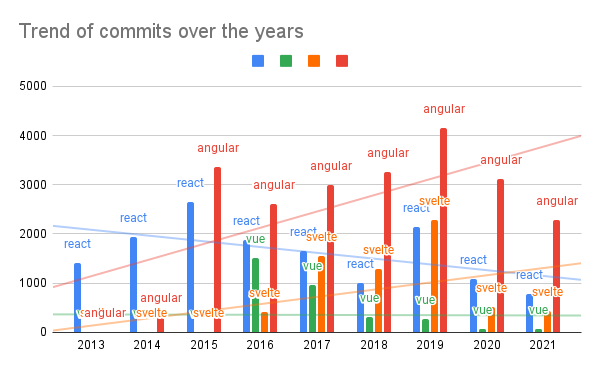
\includegraphics[scale=0.35]{trend-of-commits-over-the-years}    
\end{center}

When it comes to React, the number of commits increased for the first three years of its existence but has since declined, whereas the rate of commits for Angular has been increasing since its inception in 2015.

Vue and Svelte are the two newest frameworks as of 2016, and while Vue's contribution has been more stable in recent years, Svelte appears to outpace Vue regularly.

Even though React is the only project that has a declining trendline we don't think that is dying, if we take a look at the table provided in the section \textit{Current state of the world}, React is used by 7.6 million projects.

We can't take react outside of the context in which it was born, inside Facebook, to standardize the way that developers create user interfaces, we attribute this decline to the maturity of the framework, using the Capability maturity model \cite{cmm}, tell us that the project is at level 5, and their focus right now is to improve performance while keeping the stability of the project.

\paragraph{Trend of opened issues over the years: }
While the previous trend emphasizes how the community interacts with the project, issues are the social component in open source, at least on GitHub.

In the chart below, we used the same approach as before: we took all the data where the issues were open, grouped them by year, and put the projects next to each other to get any insights; below, we have a chart that depicts a summary of the issues over the years, and we used the following data set \cite{trend-of-open-issues-over-the-years}.

\begin{center}
    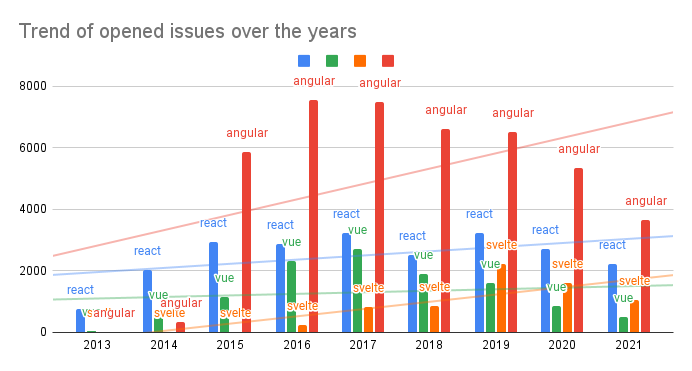
\includegraphics[scale=0.35]{trend-of-open-issues-over-the-years}    
\end{center}

From the chart we can see that angular has the most active community overall, from react we can see that we have an increasing trendline over the years, which contrast with the decline that it's perceived from the previous trend, which helps with the assumption that we make before that commit's alone are not a single representative metric that provides \textit{liveliness} to a project, Vue has a slight increase over the years and has the same trend behavior that was displayed in the previous trend, svelte seems to have an increase trendline as well, surpassing Vue community in the last 3 years.

This could indicate that, in general, all of these communities are relatively active, implying that the project is socially active.

\paragraph{Trend of unique contributors per year}
We have already seen how many contributions a project received in the form of commits and how the community interacts with one another, now we will see how big the community is by the number of unique developers who contribute to the project, and we will use the following data set \cite{trend-of-unique-contributors-per-year} to create the chart below.

\begin{center}
    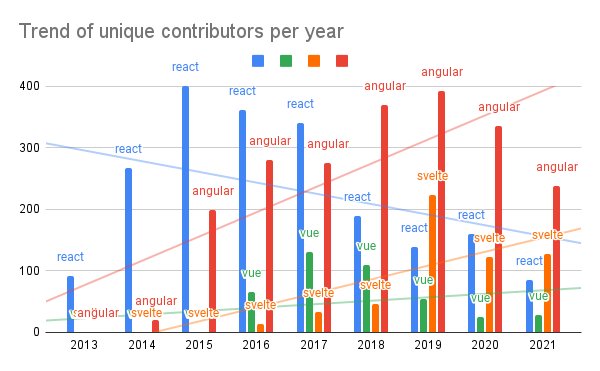
\includegraphics[scale=0.35]{trend-of-unique-contributors-per-year}    
\end{center}

From the chart we can see a decline in React from 2015 to 2021, it could be because at the beginning more developers were joining but with the pass of time the community was getting more mature and the contributions got centralized which coincide with the trend of commits over the years, angular has received an increase in unique contributors each year which is a sign that the amount of developers is growing, svelte has seen an increase in the last years and Vue has received a fairly increase of contributors since it's inception.

\subsubsection{What is the overall sentiment of the project?}
Using the following data \cite{overall-sentiment}, we will now assess each project's positive and negative sentiments.

We will see a chart below showing the percentage of positive and negative words used in each project.

\begin{center}
    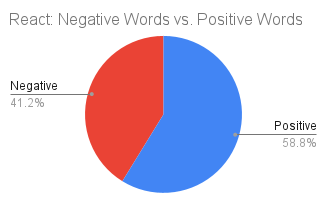
\includegraphics[scale=0.5]{react-words}    
\end{center}

In this chart we can see that react has more positive (162,415) words that represent 58.8\% compared to the negative (113,892) words, which represent 41.2\%.

\begin{center}
    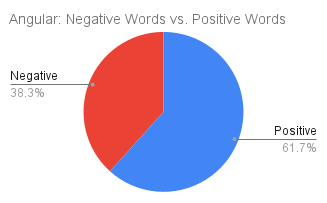
\includegraphics[scale=0.50]{angular-words}    
\end{center}

In the case of angular we have a more positive community than react with 280,779 positive words, which represents 61.7\%, compare with the 174,500 negative words which represent 38.3\%.

\begin{center}
    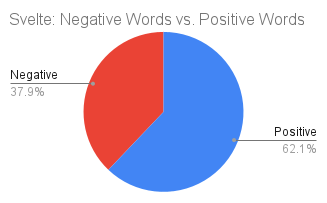
\includegraphics[scale=0.50]{svelte-words}    
\end{center}

Next, we have svelte with 35,965 positive words that represent 62.1\% and 21,948 negative words that represent 37.9\%.

\begin{center}
    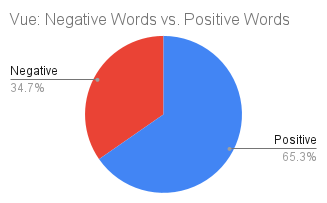
\includegraphics[scale=0.50]{vue-words}    
\end{center}

Vue has a total of 44,901 positive words, 65.3\%, and 23,821 negative words, 34.7\%.

This data suggests that all communities are positive in general, but there are significant differences between them. We will now display the most frequently used words, the top 20, using cloud words, and for each project, we will see if it gives us an indication of what the community looks like.

\begin{center}
    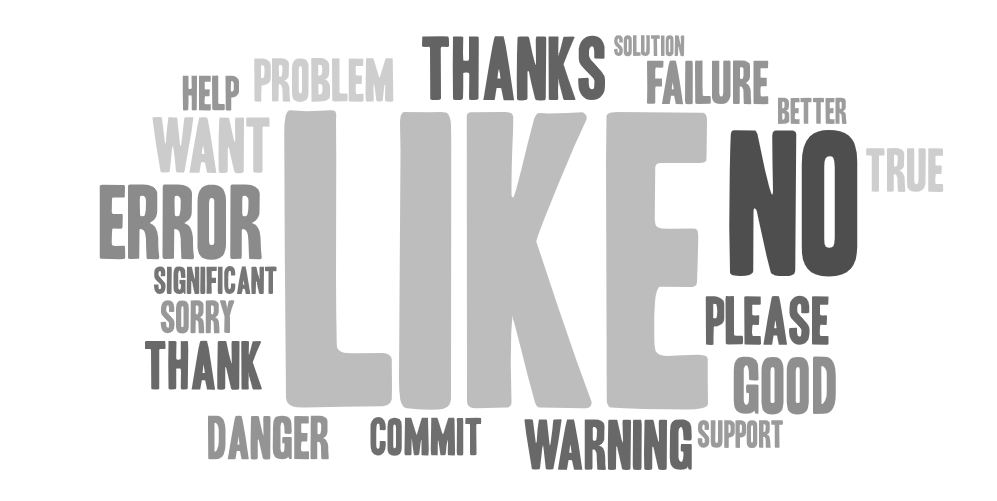
\includegraphics[scale=0.20]{react-word-cloud}    
    \textit{React}
\end{center}


\begin{center}
    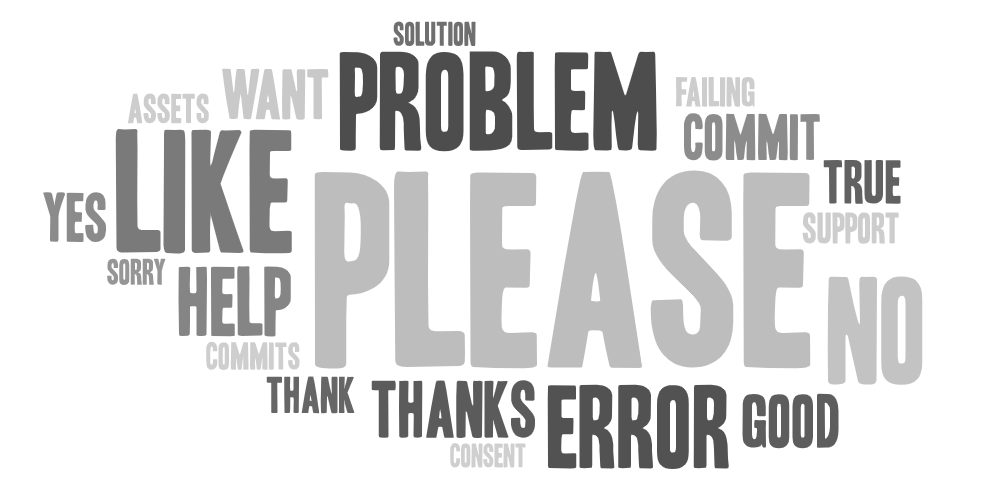
\includegraphics[scale=0.20]{angular-word-cloud}    
    \textit{Angular}
\end{center}


\begin{center}
    
\includegraphics[scale=0.20]{vue-word-cloud}    
    \textit{Vue}
\end{center}

\begin{center}
    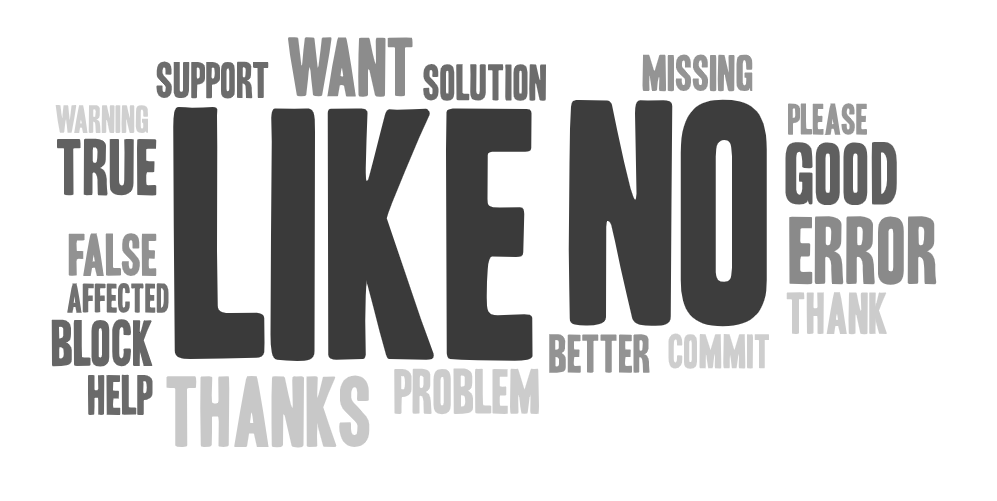
\includegraphics[scale=0.20]{svelte-word-cloud}    
    \textit{Svelte}
\end{center}

From the cloud words we can see that the most use words is \textbf{Like} and \textbf{Please}, and most uses get used accross multiple projects like \textbf{thanks}, \textbf{thank}, \textbf{good}, \textbf{no}, \textbf{problem}, which suggest that there is not a specific words that difference one community from another and overall all the communities are positive, because if we take a look at the negative words are words like \textbf{no}, \textbf{danger} or \textbf{problem} which could for fixing a particular problem.

\section{Analysis}
Compared to svelte and Vue, \textbf{React} and \textbf{Angular} have made the most significant overall contribution because they were the first while being backed by large companies React (Facebook) and Angular (Google), which drove early adoption.

In general, all the projects have an active community and the projects are being developed, and the community seems to use the same kind of word, so there isn't any bad choice from a community side.

If we are talking about impact, we would recommend Vue because it has the fewest contributors, making it easier to leave your mark on the project. However, if you want to learn new skills and have a larger community, we recommend Angular and React, which have the most contributors.

If the contributor wants to learn something new and take a different approach than the other frameworks, we recommend Svelte, but the fourth project is excellent for the metrics we establish, the "liveliness," and their communities in general.

\section{Future Work}
Even though this paper focused on the most popular front-end frameworks, the approach for the community could be expanded by including Reddit or StackOverflow.

Since this one is primarily social it could give us a view of how the community interacts outside of the scope of the project, while having the usage of the project as the main topic.

The method described in this paper could be applied to a wide variety of projects and libraries, not just for first-time contributors but also for seasoned contributors who want to contribute to a project in a specific area and have various options.
